\documentclass{article}\usepackage[]{graphicx}\usepackage[]{color}
% maxwidth is the original width if it is less than linewidth
% otherwise use linewidth (to make sure the graphics do not exceed the margin)
\makeatletter
\def\maxwidth{ %
  \ifdim\Gin@nat@width>\linewidth
    \linewidth
  \else
    \Gin@nat@width
  \fi
}
\makeatother

\definecolor{fgcolor}{rgb}{0.345, 0.345, 0.345}
\newcommand{\hlnum}[1]{\textcolor[rgb]{0.686,0.059,0.569}{#1}}%
\newcommand{\hlstr}[1]{\textcolor[rgb]{0.192,0.494,0.8}{#1}}%
\newcommand{\hlcom}[1]{\textcolor[rgb]{0.678,0.584,0.686}{\textit{#1}}}%
\newcommand{\hlopt}[1]{\textcolor[rgb]{0,0,0}{#1}}%
\newcommand{\hlstd}[1]{\textcolor[rgb]{0.345,0.345,0.345}{#1}}%
\newcommand{\hlkwa}[1]{\textcolor[rgb]{0.161,0.373,0.58}{\textbf{#1}}}%
\newcommand{\hlkwb}[1]{\textcolor[rgb]{0.69,0.353,0.396}{#1}}%
\newcommand{\hlkwc}[1]{\textcolor[rgb]{0.333,0.667,0.333}{#1}}%
\newcommand{\hlkwd}[1]{\textcolor[rgb]{0.737,0.353,0.396}{\textbf{#1}}}%
\let\hlipl\hlkwb

\usepackage{framed}
\makeatletter
\newenvironment{kframe}{%
 \def\at@end@of@kframe{}%
 \ifinner\ifhmode%
  \def\at@end@of@kframe{\end{minipage}}%
  \begin{minipage}{\columnwidth}%
 \fi\fi%
 \def\FrameCommand##1{\hskip\@totalleftmargin \hskip-\fboxsep
 \colorbox{shadecolor}{##1}\hskip-\fboxsep
     % There is no \\@totalrightmargin, so:
     \hskip-\linewidth \hskip-\@totalleftmargin \hskip\columnwidth}%
 \MakeFramed {\advance\hsize-\width
   \@totalleftmargin\z@ \linewidth\hsize
   \@setminipage}}%
 {\par\unskip\endMakeFramed%
 \at@end@of@kframe}
\makeatother

\definecolor{shadecolor}{rgb}{.97, .97, .97}
\definecolor{messagecolor}{rgb}{0, 0, 0}
\definecolor{warningcolor}{rgb}{1, 0, 1}
\definecolor{errorcolor}{rgb}{1, 0, 0}
\newenvironment{knitrout}{}{} % an empty environment to be redefined in TeX

\usepackage{alltt}

\title{Data visualisation assignment } 

\author{Zan Zver,\\ 
        student number: 18133498,\\
        total word count 2100}
\IfFileExists{upquote.sty}{\usepackage{upquote}}{}
\begin{document}

\maketitle

\newpage
  \tableofcontents
\newpage
  \listoffigures
\newpage
%--------------------------------------------------------------------------------------------------
% Abstract
%--------------------------------------------------------------------------------------------------
 \maketitle
  \newpage
    \section{Abstract} 
      New York City is one of the most populated cities on the globe. With a population large like that,        crime rate must be higher! But did it change over time? Does gender or race effect that? We have          known that people with darker skin tone get arrested more often, but is it true? Are women less           likely to be arrested? Those are some of the questions that where are answered.\vspace{5mm}
      
      But as a traveller, you might have different questions. If you go there for vacation or work, you         might want to avoid dangerous sections of the city. It is also discussed what is the most popular         month for arrests. So, if you are planning a trip to New York City, you might want to go at the           specific time.\vspace{5mm}
      
      Since our readers might be interesting to the side of the law, there are two sections for them. Two       of more advanced topics are: “jurisdictions code” and “law code”. Those two topics are presented          with some “code names” which might be a bit more applicable to advanced readers.\vspace{5mm}


%--------------------------------------------------------------------------------------------------
% Introduction
%--------------------------------------------------------------------------------------------------
  \maketitle
    \newpage
      \section{Introduction} 
        \subsection{Summarise}
          This is a report is based about crimes in New York City. Crimes are presented over time, by               perps’ diversity, law cases... Topic are presented for medium level readers. There are a couple           of topics at the end that are for advanced users.\vspace{5mm}
          
          Report has some questions that needed to be answered. Conclusions that were driven out, have              confirmed and denied to them. Some of the popular highlights that were found are listed below. 

        \subsection{Highlight}
          Overall, there are some interesting observations that can be find in the report:
          \begin{enumerate} 
            \item Fall of crime rate,
            \item Most popular crime, 
            \item Asians crime statistic.
          \end{enumerate}
      
        What is interesting is different from one person to another, therefore you (the reader) mind find         those highlights a bit boring. As they say, “everyone has different point of view” and I (writer)         hope you can find something interesting for yourself!
      
        \subsection{Aim}
        Aim of this report is to have a look on some of the most popular questions that we might have.            Well known and diverse question is that Afro American people get arrested more often due to their         skin tone.\vspace{5mm}
      
        When we see a police car, most common thought is that they are going to some place that was robbed         or someone got killed. But That is common misconception that is shown from data! 
      
        \subsection{Achievements}
        In this report, reader can find answers to some of the most popular questions. They can be                presented with map of crimes in NYC, the most common law code used, most popular arrest case over         time, etc…\vspace{5mm}
      
        Some of the questions and its theories were proven correct and some of them were proven wrong             based on the given dataset. 
      
        \subsection{Organised}
        Structure of this report is:
        \begin{enumerate} 
          \item Title
            \begin{enumerate} 
              \item	Subtitle (if applicable)
              \item	Description
              \item	Graph (graphs are on own page)
            \end{enumerate}
        \end{enumerate}
        
%--------------------------------------------------------------------------------------------------
% Motivation and objectives
%--------------------------------------------------------------------------------------------------
  \maketitle
    \newpage
      \section{Motivation and objectives} 
        Since New York City is one of the largest cities on the globe based on population, the crime rate         is increased. NYC is also one of the popular tourists’ destinations, therefore, crime rate is             increased.\vspace{5mm}

        Data is from NYC open data. This data is free and accessible to everyone. Original name is “NYPD          Arrests Data Historic”. It gets updated annually and it was made public on 11.1.2018.\vspace{5mm}

        This dataset has 5.01M rows and 18 columns.\
        Columns from dataset:
        \begin{enumerate}
          \item arrest key,
          \item arrest date,
          \item PD CD,
          \item PC DSEC,
          \item KY CD,
          \item OFNS DESC,
          \item law code,
          \item law cat CD,
          \item arrest boro,
          \item arrest precinct,
          \item jurisdiction code,
          \item age group,
          \item perp sex,
          \item perp race,
          \item x coord CD,
          \item Y coord CD,
          \item latitude,
          \item longitude.
        \end{enumerate}

%--------------------------------------------------------------------------------------------------
% Questions about dataset
%--------------------------------------------------------------------------------------------------
  \maketitle 
     \newpage   
        \subsection {Questions about dataset}
          This is a representation of questions that we are looking to be answered with expected results:
          \begin{enumerate}
            \item	
              Q: How are arrest cases doing through the years?\\
              E: Since population has gone up, arrest percent hasn’t changed.
            \item
              Q: Are there specific months where arrests are higher?\\
              E: In the summer arrests might be higher due to people being on holidays
            \item
              Q: What is the reason people are most likely to get arrested for?\\
              E: Assumption is that most people get arrested for stealing items.
            \item
              Q: Are top arrest cases changing over the years?\\
              E: They are changing due to people discovering easier ways to do illegal stuff.
            \item
              Since people are different, how are factors applied to them:
              \begin{enumerate}
                \item
                  Q: Does the skin tone matter?\\
                  E: It does, due to racism still being a thing. 
                \item
                  Q: Does gender matter?\\
                  E: Yes, more man are arrested than woman. 
                \item
                  Q: Does age matter?\\
                  E: Assumption is that younger people are more likely to be arrested.
              \end{enumerate}
            \item
              Q:  Top arrest locations.\\
              E: No assumption was made.
            \item
              Q: Who is most likely to arrest a person based on jurisdiction responsible?\\
              E: No assumption was made
            \item
              Q: What law code have been used most likely and why?\\
              E: No assumption was made
          \end{enumerate}
      
       \noindent Q- question\\
        E- expectation 
          
%--------------------------------------------------------------------------------------------------
% Experimental Results
%--------------------------------------------------------------------------------------------------
  \maketitle
    \newpage
      \section{Experimental Results} 
      This section is research based. There is a list of questions that is being answered. It is structurd       as explanation about the question, graphs fallow afterwards on the new page. 

%--------------------------------------------------------------------------------------------------
% Number of arrests through  the years
%--------------------------------------------------------------------------------------------------
    \newpage
      \subsection{Number of arrests through  the years}
        Over the years New York’s population has gone up for 663000 since 2006 (4\%increase). So, did             crime gone up as well since population did? 
        In 2006, there was 12500 arrest cases. If we increase this number by 4\% every year estimated             arrests are 21646 by 2019. But that hasn’t happened! In 2019, there were only 8750 arrests. This          is 0.7\% less! The spike was in the middle of 2010, afterwards crime rate has gone down. In first         quarter of 2018, we can see that crime rate is going up.\
        
        But when do those arrest happen? Since most of the people go to holidays in the summer, is this           the best time for get in trouble? The answer is no! The summer is not the busies for criminals,           March is!
        
        \begin{figure}[hbtp]
          \caption{Arrests over time}
\begin{knitrout}
\definecolor{shadecolor}{rgb}{0.969, 0.969, 0.969}\color{fgcolor}
\includegraphics[width=\maxwidth]{figure/unnamed-chunk-1-1} 

\end{knitrout}
        \end{figure}
          
        \begin{figure}[hbtp]
          \caption{Comparison of arrests over years}
\begin{knitrout}
\definecolor{shadecolor}{rgb}{0.969, 0.969, 0.969}\color{fgcolor}
\includegraphics[width=\maxwidth]{figure/unnamed-chunk-2-1} 

\end{knitrout}
        \end{figure}
          
        \begin{figure}[hbtp]
          \caption{Comparison of arrests over months}
\begin{knitrout}
\definecolor{shadecolor}{rgb}{0.969, 0.969, 0.969}\color{fgcolor}
\includegraphics[width=\maxwidth]{figure/unnamed-chunk-3-1} 

\end{knitrout}
        \end{figure}
          
        \begin{figure}[hbtp]
          \caption{Months compared}
\begin{knitrout}
\definecolor{shadecolor}{rgb}{0.969, 0.969, 0.969}\color{fgcolor}
\includegraphics[width=\maxwidth]{figure/unnamed-chunk-4-1} 

\end{knitrout}
        \end{figure}

%--------------------------------------------------------------------------------------------------
% Top arrest cases
%--------------------------------------------------------------------------------------------------
  \maketitle
    \newpage
      \subsection{Top arrest cases}
      People get arrested for all kinds of stuff. But does it repeat?\
      The answer is, yes!\
      From 2006 and 2012 top arrest case was possession of Marijuana. This is interesting, because in 2014       Marijuana was legalized for medical use and in 2019 laws changed a bit. For up to 28 grams, people        are now fined for up to 50\$.\
      But if they have up to 56 grams, they are fined up to 200\$. This combination lowered number of           arrests! Some countries in US have already legalized Marijuana fully, therefore, this arrest case is       going to be declining over the future.
      
    \newpage
      \begin{figure}[hbtp]
        \caption{Top 5 arrest cases}
\begin{knitrout}
\definecolor{shadecolor}{rgb}{0.969, 0.969, 0.969}\color{fgcolor}
\includegraphics[width=\maxwidth]{figure/unnamed-chunk-5-1} 

\end{knitrout}
      \end{figure}
      
      \begin{figure}[hbtp]
        \caption{Top arrest cases over time}
\begin{knitrout}
\definecolor{shadecolor}{rgb}{0.969, 0.969, 0.969}\color{fgcolor}
\includegraphics[width=\maxwidth]{figure/unnamed-chunk-6-1} 

\end{knitrout}
      \end{figure}
      
%--------------------------------------------------------------------------------------------------
% Diversity
%--------------------------------------------------------------------------------------------------
  \maketitle
    \newpage
      \subsection{Diversity}
        In this section, we are going through: 
        \begin{enumerate}
          \item
            Race,
          \item
          	Gender,
          \item
          	Age.
        \end{enumerate}
  
        Since racism is still a thing over the years, we can see that top arrest people are with black            skin. But their arrest cases are lowering as normal. But there is one race that is not following          the graph. As it seems, Asians got arrested more in 2018 than in 2006!\

        Another factor is race. Is it true that man are more likely to be arrested? The answer is yes! Man         are 83\% more likely to be arrested than woman. But there is something interesting in the graph.          Man’s arrest cases are have fallen more drastically than women’s!

  \newpage
    \begin{figure}[hbtp]
      \caption{Comparison between races}
\begin{knitrout}
\definecolor{shadecolor}{rgb}{0.969, 0.969, 0.969}\color{fgcolor}
\includegraphics[width=\maxwidth]{figure/unnamed-chunk-7-1} 

\end{knitrout}
    \end{figure}
            
    \begin{figure}[hbtp]
      \caption{Comparison between gender}
\begin{knitrout}
\definecolor{shadecolor}{rgb}{0.969, 0.969, 0.969}\color{fgcolor}
\includegraphics[width=\maxwidth]{figure/unnamed-chunk-8-1} 

\end{knitrout}
    \end{figure}
          
    \begin{figure}[hbtp]
      \caption{Comparison  between age}
\begin{knitrout}
\definecolor{shadecolor}{rgb}{0.969, 0.969, 0.969}\color{fgcolor}
\includegraphics[width=\maxwidth]{figure/unnamed-chunk-9-1} 

\end{knitrout}
    \end{figure}

%--------------------------------------------------------------------------------------------------
% Dangerous neighbourhoods, do they expend or shrink?
%--------------------------------------------------------------------------------------------------
  \maketitle
    \newpage
      \subsection{Dangerous neighbourhoods, do they expend or shrink?}
        New York has 5 boroughs:
          \begin{enumerate}
            \item
              The Bronx,
            \item
            	Staten Island,
            \item
            	Queens,
            \item
            	Brooklyn,
            \item
              Manhattan. 
          \end{enumerate}
              
        If we have a look, Staten Island and Queens look the safest in terms of arrest cases. But                 Manhattan and Brooklyn are indicated as the most crime related cities. 

        Looking at maps, we can see that there are black dots drown on the map. The darker they are, more         arrests have been indicated at that location. These graphs can help tourists locate where to be in         New York City. People that are interested in investing to properties or moving into new apartment         can find this useful as well! Sections with heavier crime rates are darker!
                 
          \begin{figure}[hbtp]
            \caption{Map of Bronx}
              \hspace*{-7.7cm} 
                \includegraphics[scale=0.22]
                  {/Users/zanzver/Desktop/DataVIs/map/Bronx.png}
          \end{figure}
            
          \begin{figure}[hbtp]
            \caption{Map of Brooklyn}
              \hspace*{-7.7cm} 
                \includegraphics[scale=0.22]
                {/Users/zanzver/Desktop/DataVIs/map/Brooklyn.png}
          \end{figure}
            
          \begin{figure}[hbtp]
            \caption{Map of Manhattan}
              \hspace*{-7.7cm} 
                \includegraphics[scale=0.22]
                  {/Users/zanzver/Desktop/DataVIs/map/Manhattan.png}
          \end{figure}
              
          \begin{figure}[hbtp]
            \caption{Map of Queens}
              \hspace*{-7.7cm} 
                \includegraphics[scale=0.22]
                  {/Users/zanzver/Desktop/DataVIs/map/Queens.png}
          \end{figure}
            
          \begin{figure}[hbtp]
            \caption{Map of Staten Island}
              \hspace*{-7.7cm} 
                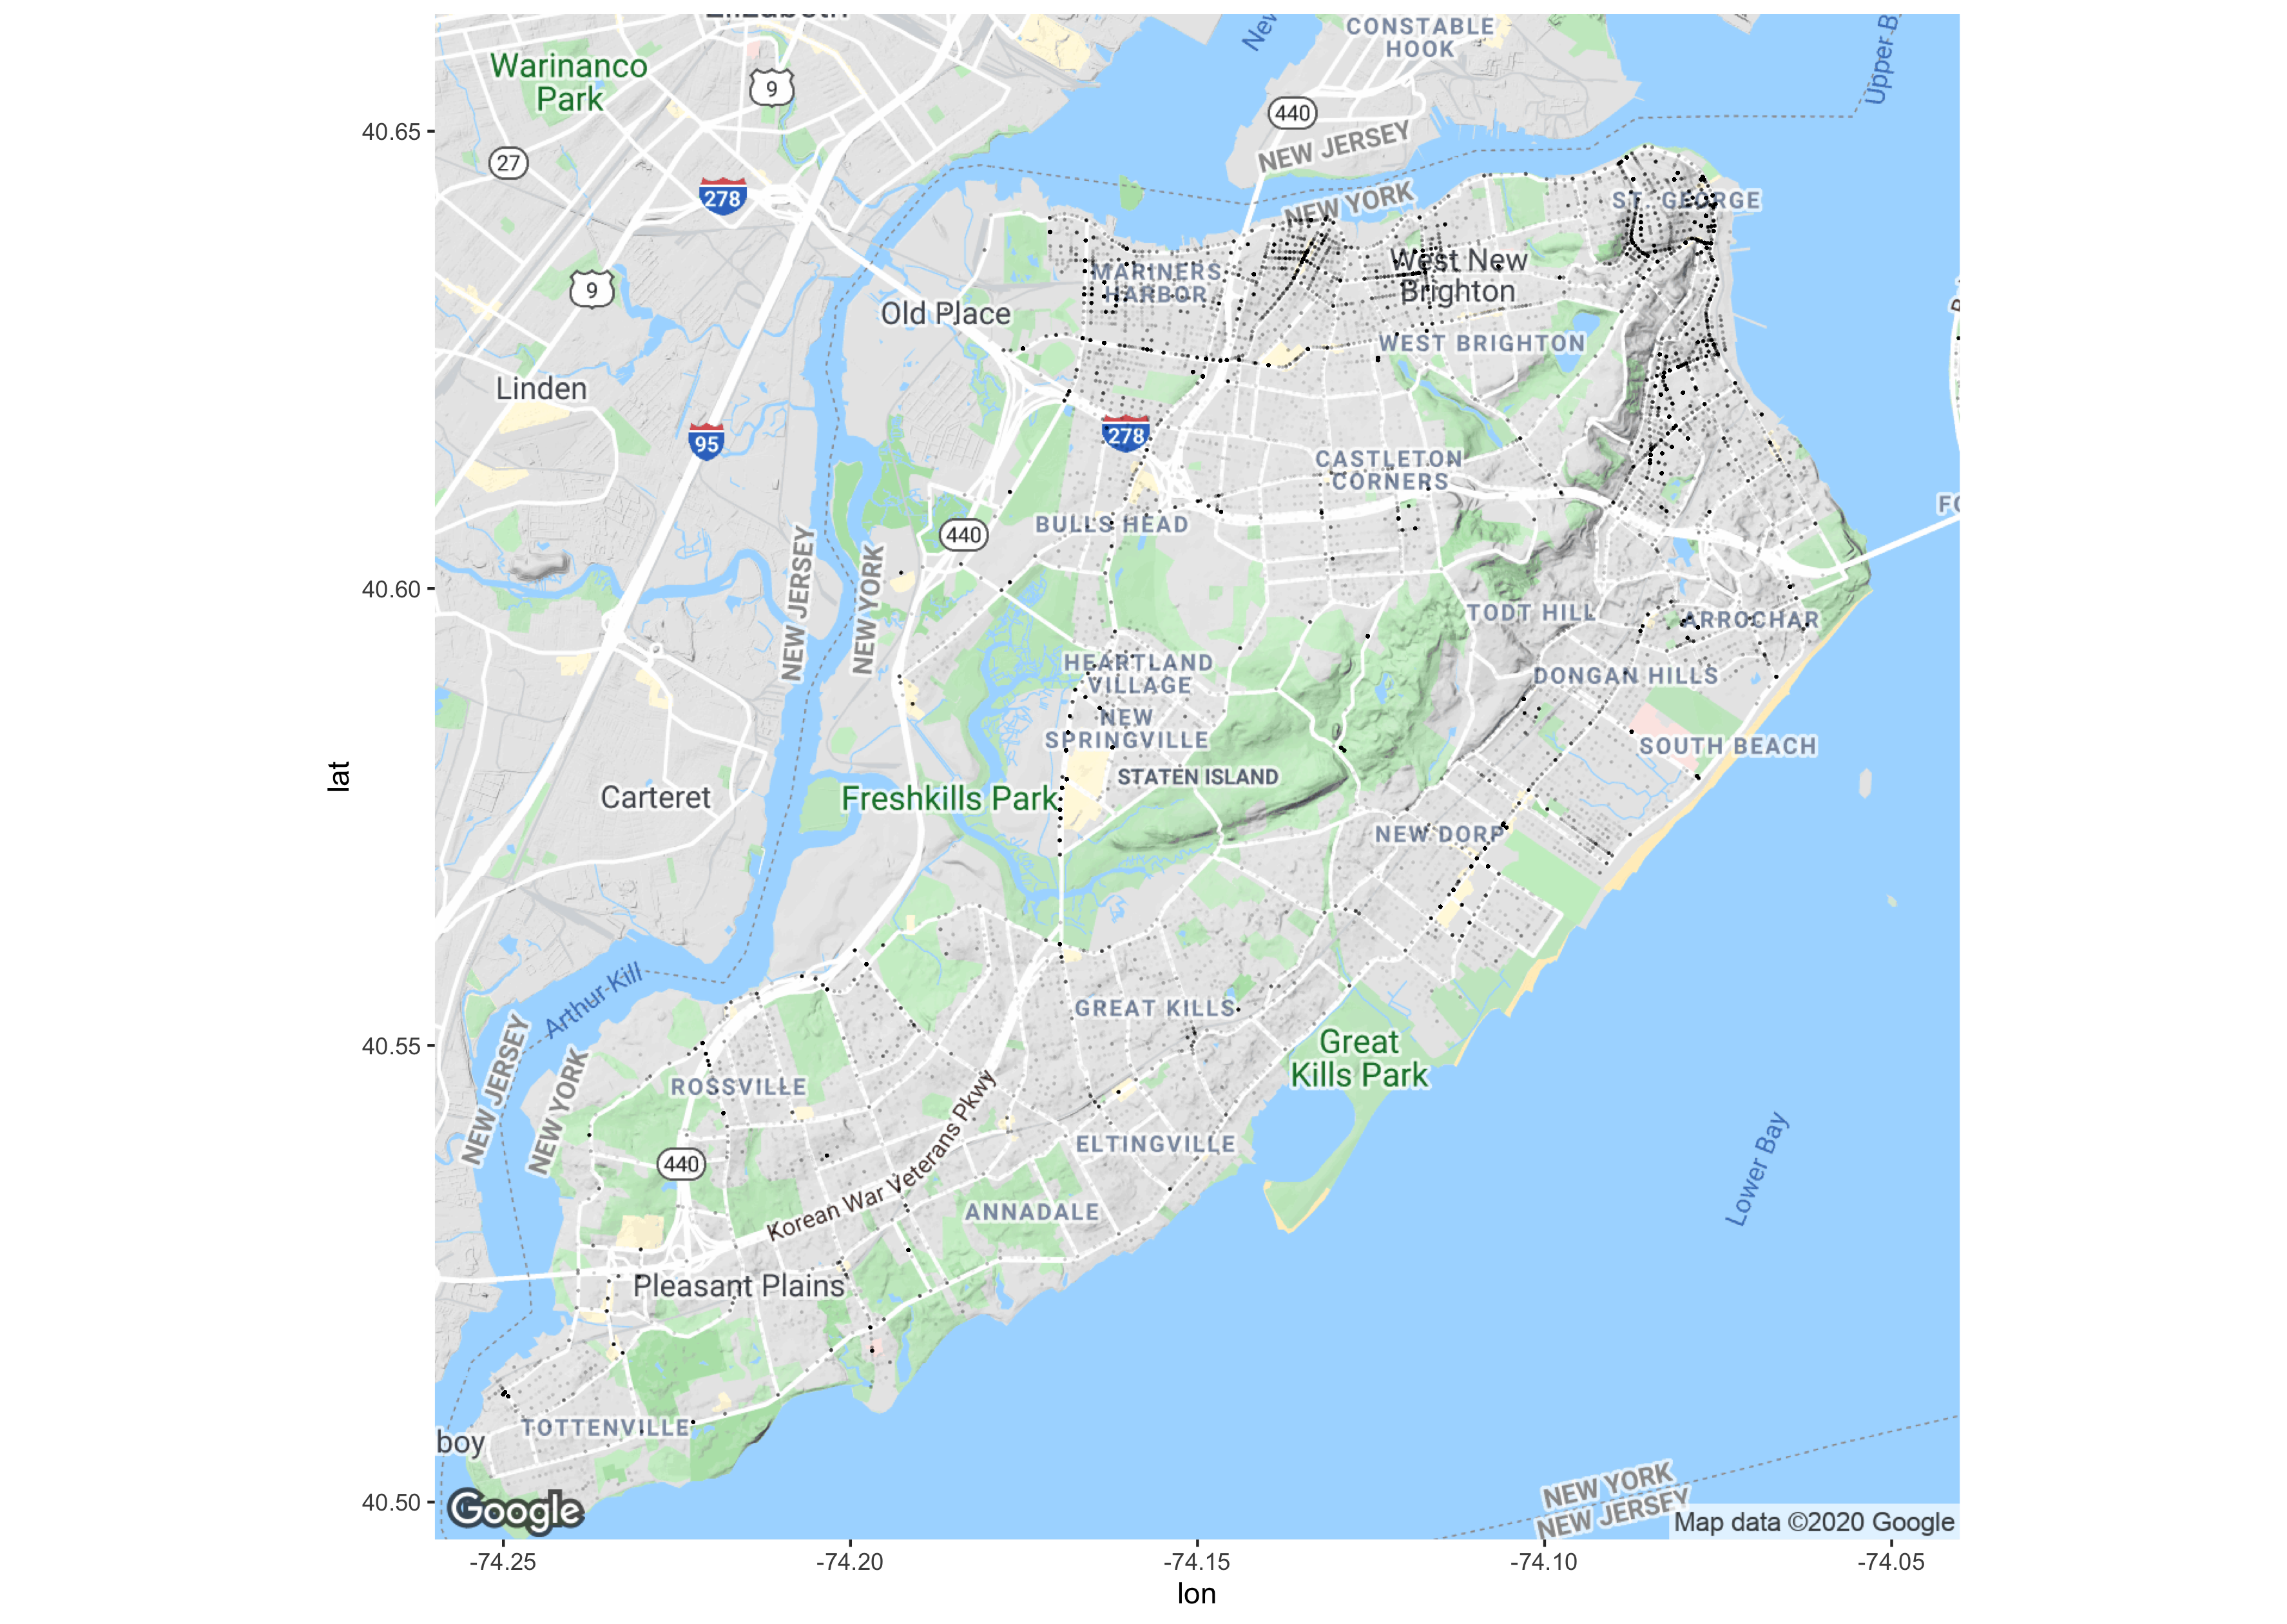
\includegraphics[scale=0.22]
                  {/Users/zanzver/Desktop/DataVIs/map/StatenIsland.png}
          \end{figure}

%--------------------------------------------------------------------------------------------------
% Who is most likely to arrest a person based on jurisdiction responsible?
%--------------------------------------------------------------------------------------------------
  \maketitle
    \newpage
      \subsection{Who is most likely to arrest a person based on jurisdiction responsible?}
      By looking the graphs, jurisdiction responsible with code 0 stands out the most! It Has almost 4          minion occurrences, when codes 1,2,3 and 97 together are less then million!\

      If a comparison is done to law code, we can see that law code and jurisdiction are not linked. This       was an interesting result due to expectations that they would be at list similar to some extent.\

      Unfortunately, the data was not on the internet nor was provided with dataset. So, explanation is         missing. Readers with more advanced knowledge in law are most likely to have a deeper understanding       about it.

        \begin{figure}[hbtp]
          \caption{Jurisdiction code used}
\begin{knitrout}
\definecolor{shadecolor}{rgb}{0.969, 0.969, 0.969}\color{fgcolor}\begin{kframe}


{\ttfamily\noindent\bfseries\color{errorcolor}{\#\# Error in file(file, "{}rt"{}): cannot open the connection}}\end{kframe}
\includegraphics[width=\maxwidth]{figure/unnamed-chunk-10-1} 

\end{knitrout}
        \end{figure}
        
%--------------------------------------------------------------------------------------------------
% What law code have been used most likely and why?
%--------------------------------------------------------------------------------------------------
    \newpage
      \subsection{What law code have been used most likely and why?}
        Top 3 arrest codes:
        \begin{enumerate}
          \item
            PL (Penal Law [criminal law]),
          \item
            VTL (Vehicle and Traffic Law),
          \item
          	LOC (General Violation Of Local Law).
        \end{enumerate}

        If we have a look on the graph, PL is top value by a lot! But why? After deeper dive into                 description, it gives us that PL covers most of the top arrest cases that we have. On the top, PL         has the widest range of laws. Therefore the result is the most common use of this law code! If we         compare VTL and LOC to PL, we can see that VTL covers more specific vehicle cases and LOC is for          smaller law cases.\

        Law codes in this section can explain a brother view of arrest types that are applied to the              people breaking the law. This is one of the topics that advanced readers might take a deeper              understanding of it, but it is worth mentioning.


        \begin{figure}[hbtp]
          \caption{Most common law code}
\begin{knitrout}
\definecolor{shadecolor}{rgb}{0.969, 0.969, 0.969}\color{fgcolor}
\includegraphics[width=\maxwidth]{figure/unnamed-chunk-11-1} 

\end{knitrout}
        \end{figure}

%--------------------------------------------------------------------------------------------------
% Summary
%--------------------------------------------------------------------------------------------------
  \maketitle
    \newpage
      \section{Summary}
      This report has covered crimes that were done in New York City from years of 2006 and to the end of       2018. As we have gone through the report and answered the questions, we have managed to confirm some       thoughts and delight others.\
      
      Observations that were find interesting in the report have come to the conclusion:
      \begin{enumerate}
        \item
            Fall of crime rate,\
      	    Despite of growth of population (4\%) in New York City, the crime rate has gone down by the               7\%.
        \item
            Most popular crime, \
            Reasons for crime are always changing. From drugs, money laundering and current being assault.             But there is a suspicion that cybercrime is going to be on the top due to the increase usage              of computers.
        \item
            Asians crime statistic.\
            There was a downfall of crime in the fallowing years. This is noted with every race, accept               Asians. Their crime rates have gone up over time, which is interesting.

      \end{enumerate}
      
      Findings:
      \begin{enumerate}
        \item	
          Q: How are arrest cases doing through the years?\\
          E: Since population has gone up, arrest percent hasn’t changed.\\
          F: Crime rate has gone down despites population going up.
        \item
          Q: Are there specific months where arrests are higher?\\
          E: In the summer arrests might be higher due to people being on holidays.\\
          F: This was proven wrong. Most of the arrest are not done in that time.
        \item
          Q: What is the reason people are most likely to get arrested for?\\
          E: Assumption is that most people get arrested for stealing items.\\
          F: This was proven wrong. Top arrest case was people having Marijuana on them.
        \item
          Q: Are top arrest cases changing over the years?\\
          E: They are changing due to people discovering easier ways to do illegal stuff.\\
          F: Assumption was proven correct.
        \item
          Since people are different, how are factors applied to them:
          \begin{enumerate}
            \item
              Q: Does the skin tone matter?\\
              E: It does, due to racism still being a thing.\\
              F: Unfortunately, assumption was true, but people with black skin tone are getting                       arrested less over time.
            \item
              Q: Does gender matter?\\
              E: Yes, more man are arrested than woman.\\
              F: This was proven true, more man were arrested than women!
            \item
              Q: Does age matter?\\
              E: Assumption is that younger people are more likely to be arrested.\\
              F: This is up to viewers opinion. Ages 25-44 have the most arrests but ages from 18-24 and                <18 combined are close to 25-44! 
          \end{enumerate}
        \item
          Q:  Top arrest locations.\\
          E: No assumption was made.\\
          F: Staten Island and Queens are the safest.
        \item
          Q: Who is most likely to arrest a person based on jurisdiction responsible?\\
          E: No assumption was made.\\
          F: Code 0 was used the most.
        \item
          Q: What law code have been used most likely and why?\\
          E: No assumption was made.\\
          F: PL (Penal Law [criminal law]) code was used the most due to its description.
      \end{enumerate}
      
      
      \noindent Q- question\\
      E- expectation\\
      F- findings \vspace{5mm}

      There is still room for improvement at the end, since new questions can be asked based on new research applied to this.

%--------------------------------------------------------------------------------------------------
% References
%--------------------------------------------------------------------------------------------------
  \maketitle
    \newpage
      \section{References}
        FindLaw's team (2020). New York Marijuana Laws. FindLaw
        Available at:
        https://statelaws.findlaw.com/new-york-law/new-york-marijuana-laws.html
        [Accessed 22 May. 2020].\vspace{5mm}

        Wikipedia (unknown). Legality of cannabis by U.S. jurisdiction. Wikipedia
        Available at:
        https://en.wikipedia.org/wiki/Legality\_of\_cannabis\_by\_U.S.\_jurisdiction
        [Accessed 22 May. 2020].\vspace{5mm}

        DCJS (2020). DCJS Coded Law File. Division of Criminal Justice Services
        Available at: 
        https://www.criminaljustice.ny.gov/crimnet/ccman/codedlawmanual.pdf
        [Accessed 23 May. 2020].\vspace{5mm}
        
        Unknown (unknown). Criminal Court Summonses in New York City. Marijuana-arrests. 
        Available at:
        http://marijuana-arrests.com/docs/Criminal-Court-Summonses-in-NYC--CUNY-Law-School-April-24-2014.pdf
        [Accessed 24 May. 2020].\vspace{5mm}

\end{document}
